\documentclass[html]{report}    % Specifies the document style.
\usepackage{graphicx}
\usepackage{verbatim}
\usepackage{tabularx}
\usepackage{booktabs}
\usepackage{multirow}
\usepackage{marginnote}
\usepackage{caption}
\usepackage{color}
\usepackage{subcaption}

%\usepackage[top=1.5cm, bottom=1.5cm, outer=5cm, inner=2cm, heightrounded, marginparwidth=2.5cm, marginparsep=2cm]{geometry}
\usepackage{amsmath}  % allows to use some of math functions
\usepackage{breqn}    % breaks equations in parts when needed

\title{Multi-Agent Systems Project}  % Declares the document's title. 
\author{Panagiotis Chatzichristodoulou and Kirill Tumanov} 
%\date{November 29,2013}   % Deleting this command produces today's date.

\begin{document}           % End of preamble and beginning of text.

\maketitle                 % Produces the title.
\section{Introduction}
\subsection{Abstract}
This paper addresses the implementation of an intelligent negotiation agent. Furthermore, it discusses and analyses the results obtained from the experiments that were performed as a part of the work. The agent was developed based on the \textit{Genius} software platform, released by Delft University in 2009. Genius introduces an environment where agents can negotiate within different domains - discrete or continuous. Genius is a modern standard in the agent negotiation platforms. Furthermore, in accordance to the \textit{ANAC'2013} guidelines, the agent is based on the~\textit{BOA} (Bidding Strategy, Opponent Model, Acceptance Strategy) framework~\cite{genius}. The work was performed as a practical part of the Multi-agent Systems course at Maastricht University. 

\subsection{Framework}
Agents in the Genius platform can either be standalone, or belong to the BOA framework. A single-entity agent can include all the required modules in itself or use the BOA components instead. Some additional helper classes can exist outside of the main agent class. A BOA agent implements the four models needed independently, and its modular architecture makes the agent more versatile and extendable. The Fig.~\ref{ANAC BOA} depicts how the BOA components are related between themselves.
\begin{figure}[htbp]
	  \caption{Scheme of a BOA framework}
	  \centering
	    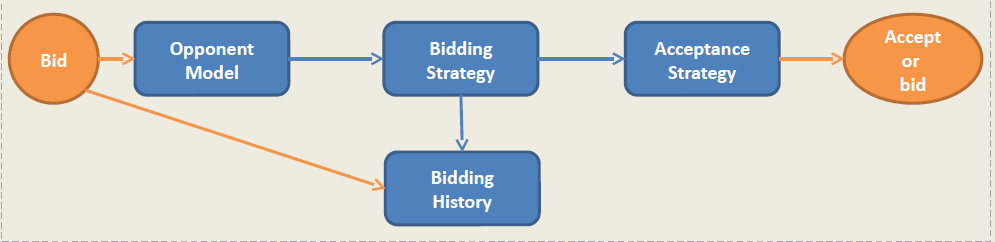
\includegraphics[width=1\textwidth]{fourmodels}
	  \label{ANAC BOA}
\end{figure}

\subsection{Agent summary}
The agent described in this paper was named \textit{NegoAgent}. It behaves as a self-interested negotiator, meaning that it seeks to maximize its utility without taking into account the opponent's score, or the social welfare. However, it takes into account the discount factor $\delta$, and keeps track of the negotiation time in order to receive the highest utility possible. The agent is not going to accept not reasonable offers - it believes that "no deal is better than a bad deal", but when possible it tries to achieve a "win-win" compromise with an opponent. Overall, the agent is not tied to any specific domain or opponent behavior type, on contrary it tries to be adaptive to the challenges to its benefit.

A description of the BOA components used for the agent development is given in subsequent sections, followed by modeling results and discussion.

\section{Bids Offering Strategy}
Agent's bid offering strategy was implemented as time-dependent (TD). The \texttt{NegoAgent_TDOffering} class requires two user parameters: $P_{min}$ and $P_{max}$ which specify the lower and upper bounds for the bids agent is to propose. In the current version of the agent these values were kept equal to $0$ and $0.99$ respectfully. No experimentation was done on changing these values, it may be the case that some alterations in specific negotiation domains are beneficial, however this topic is left for an additional research.

Offering strategy introduces two methods used in the agent: \texttt{isNash} and \texttt{countUniqueBids}. First one is a simple implementation of the two-factor (due to the number of negotiating parties) maximization algorithm. An idea behind it is in finding a Nash equilibrium point, where none of the parties can obtain a higher utility at no cost to any other party. This particular implementation does not claim to be optimal, but it produced sufficiently good results for the agent at this stage of development. The pseudo-code of the  \texttt{isNash} method is given as follows:
\begin{verbatim}
double nashsum;
boolean isNash(){
    bid = getOpponentLastBid();		
    if (bid != null) {
        temp = bid.getMyUtility() + bid.getOppenentUtility();
        if (temp < nashsum 
           && bid.getOppenentUtility() < bid.getMyUtility()) {
            return true;			
        }
        nashsum = temp;
    }		
    return false;
}
\end{verbatim}
Here \texttt{nashsum} stores a previously found maximum combined utility result to compare the last opponent's bid against. When \texttt{nashsum} becomes less than the last bid combined utility, then Nash is found and true is returned. An additional limit in the opponent's and agent's utilities is set to ensure, that Nash bid was proposed by the opponent, and not by the agent itself.

The second method \texttt{countUniqueBids} is implemented to find and count all the opponent's non-equal bids as well as calculate a total sum of all proposed bids. A pseudo-code of the method is given below.
\begin{verbatim}
uniquebids;
double bidsum;
countUniqueBids() {
    int count = 0;
    bid = getOpponentLastBid();	
    if (getOpponentBidHistory().size() == 1) {
        uniquebids.add(bid.getMyUtility());
        bidsum += bid.getMyUtility();
    }
    else {
        for (uniquebid : uniquebids) {
            if (uniquebid != bid.getMyUtility()) {
                count ++;
            }
        }
        if (count == uniquebids.size()) {
            uniquebids.add(bid.getMyUtility());
            bidsum += bid.getMyUtility();
        }
    }
}  
\end{verbatim}
This method is called every time an opponent proposes a new bid. As a result a list of \texttt{uniquebids} representing agent's utility values, \texttt{bidsum} value of all bids and \texttt{count} are stored and used for further calculations.

The main procedure of the agent's bidding strategy is \texttt{determineNextBid} which relies on a time-dependent function \texttt{p(t)}. For this work we introduce a novel TD function, results of which are determined by the values received from the methods described above. The following is a pseudo-code of the \texttt{p(t)} implementation.
\begin{verbatim}
int bidsThreshold ;
double timeThreshold;
double p(double t) {
    countUniqueBids();
    double ft = calculateF(t);
    double time = getTime();
    if (getNumberOfPossibleBids() < bidsThreshold) {
        if (time > timeThreshold) {
            ft += getOpponentLastBid.getMyUtil()/(1 - time);
        }
    }
    pt = Pmin + (Pmax - Pmin) * (1 - ft);
    return pt;
}
\end{verbatim}
Here \texttt{pt} is used only for adjustment of the \texttt{ft} result based on the $P_{min}$ and $P_{max}$ bid bounds discussed at the beginning of the section. The most interesting part is a calculation of \texttt{ft}:
\begin{equation} \label{1}
	f(t) = \begin{cases}
			df(\sin(-n\cdot e^{t\cdot df})+(\frac{1}{df}-1))\cdot\log(t\cdot df+1)\cdot\frac{sum}{ubs}t &\text{if ubs$>$1 and !isNash(),}\\
			\frac{df}{2}(\sin(-n\cdot e^{t\cdot\frac{df}{2}})+(\frac{2}{df}-1))\cdot\log(t\cdot \frac{df}{2}+1)\cdot\frac{sum}{ubs}t &\text{if ubs$>$1,}\\
			df(\sin(-n\cdot e^{t\cdot df})+(\frac{1}{df}-1))\cdot\log(t\cdot df+1) &\text{otherwise.}
			\end{cases}
\end{equation}
where $df$ - a division factor in a range $\{0\dots1\}$, $n$ - number of issues a negotiation is about, $t$ - a normalized representation of time, $sum$ - a total sum of all opponent's bids at the moment of $t$ (afore-referred as a \texttt{bidsum}), $ubs$ - number of unique opponent's bids at the moment of $t$ (a size of an afore-referred list of \texttt{uniquebids}).

The function $f(t)$ was designed so that it allows modification of bid offering dependent on the negotiation status. If opponent proposes more non-equal bids of a decent utility for an agent, then agents offers new bids more cautious - simulation of waiting for the best opponent's offer. On contrary, when opponent proposes a few non-equal bids, agent tries to provoke an opponent for cooperation, by offering more new bids. In addition, a fact of Nash equilibrium reach by an opponent is treated as a trigger to loose agent's own offering, and to start biding more actively. It is done in order to prevent an opponent from unnecessary utility losses, whilst it is likely that agent's own score is not going to be lowered. Finally, increase of $t$ during the negotiation process unveils more new bids to offer, and $n$ ensures that the offering will be domain-dependent.

Referring back to the pseudo-code of \texttt{p(t)}, in case of a very limited utility space (\texttt{getNumberOfPossibleBids()~$<$~bidsThreshold}) and negotiation time running out (\texttt{time > timeThreshold}), agent begins to concede by increasing the $f(t)$ value proportionally to the remaining time $(1-t)$. This allows to reach an agreement, instead of loosing all the utility. However, note that when opponent follows a non-cooperative strategy, this approach will not be of help.                

\section{Acceptance Strategy}
              
An Acceptance Strategy of the agent was based on the ABiNeS strategy~\cite{abines} and on a TD sigmoid function. 

\subsection{ABiNeS}
This module introduces an acceptance threshold $\ell$. The value of $\ell$ corresponds to the agent's concession degree and is modified during the negotiation. This change is based on the previous results of the negotiation as well as on the domain.

The agent is build as a self-interested agent and will be more concessive as the deadline of $t=1$ approaches. The acceptance threshold should always be higher than the utility agent can obtain at deadline. Therefore, the threshold should never be lower than the \(Utility_{max}\cdot discount_{time-1}\), where \( Utility_{max}\) is the maximum score the agent can achieve without taking into account the discount factor. In contrast, if it takes the agent too long to reach an agreement, it may receive very low utility due to the influence of a discount factor even if the agreed outcome proposes a high utility. 

To address the issue factor $\lambda$ is introduced. It is used to balance between exploring and exploiting the negotiating partner. More formally, when time is smaller than $\lambda$, it should be modified to gradually converge to \( Utility_{max}\cdot discount_{time-1}  \). So the $\ell$ is defined as follows:

\begin{equation} \label{2}
	\ell =	\begin{cases}
	    	u^m -(u^m-	u^md^t)(t/\lambda)^a  & \mbox{if } t < \lambda, \\
	   		u^m d^t & \mbox{if } t \geq \lambda.
			\end{cases}
\end{equation}

\begin{equation} \label{3}
	\lambda =	\begin{cases}
	   		  	\lambda = \lambda_0 + (1-\lambda_0)^b &  \mbox{if } t==0,\\
	       		 \lambda = \lambda + w(1-\lambda_0)\sigma^{tc} & \mbox{if } 0<t\leq1.\\
				\end{cases}
\end{equation}
So as time increases, $\ell$ slowly decreases, and as time reaches $\lambda$, $\ell$ is set to \( Utility^{max}\cdot discount^{time} \). Graphical representation of the process is presented in Fig.~\ref{2}. Here $a<1$ is a user-specified constant value, and notable are values of $b$ and $c$ which define the curvature of nonlinear piece, specifically they set a lower bound of an acceptance threshold. This fact is crucial for the strategy's implementation, as both $b$ and $c$ values should be domain-dependent in order to adequately reflect the setup features and prevent early acceptance of non-desirable offers from an opponent. Generally~$b>1$~and~$c>1$. In this work they were defined as follows:
\begin{dmath} \label{4}	
	\begin{cases}
		b = ol \cdot \theta_1\cdot (of - mf) \cdot (1 - t) \\
		c = ol \cdot \theta_2\cdot (of - mf) \cdot (1 - t), \text{and}
	\end{cases}
\end{dmath}
\begin{dmath} \label{5}	
	\begin{cases}
		b = b\cdot(1 - usmin) \\
		c = c\cdot(1 - usmin),
	\end{cases}
\end{dmath}
where $ol$ - an opponent's last bid utility, $of$ and $mf$ - opponent's and the agent's first bid utilities respectfully, and $\theta_{1,2}$ - coefficients with values $>1$. Formula~\ref{5} is used for $b$ and $c$ values normalization within a given domain. $usmin$ - is the agent's minimum possible utility in a given utility space.

\begin{figure}[htbp]
	\caption{Change of $\ell$ over time}
	\centering
	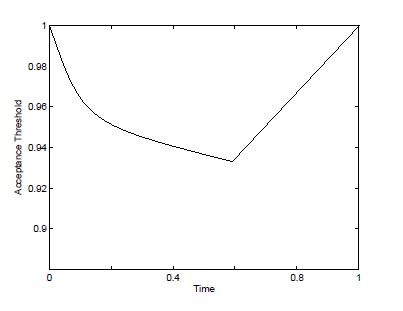
\includegraphics[width=0.5\textwidth]{ell}
	\label{2}
\end{figure}

An acceptance condition is a function of the history of the previous negotiations, the current acceptance threshold, and the outcome of the negotiation at time $t$. The agent will accept a proposal $\pi$ if it receives utility bigger than his current threshold, or his next-bid to propose utility. However this classic approach is not flexible enough when dealing with a strong opponent. An agent to be able to accept reasonable $\pi$ also need to be willing to concede more, then it would normally consider reasonable. To do so the agent needs to take into account its opponent's behavior, namely, identify how actively is an opponent bidding in order to reach an agreement. For this purpose method \texttt{countUniqueBidsAtPeriod} was introduced. It is to calculate a number of unique bids within a given time frame. The method's pseudo-code is shown below.
\begin{verbatim}
countUniqueBidsAtPeriod(double t1, double t2) {
    if (getOpponentBids().filterByTime(t1, t2).size() != 0) {
        for (bidInPeriod : bidsInPeriod) {
            ub.add(bid);
        }
        ub.removeDuplicates();
        return ub.size();
    }
    return 0;
}
\end{verbatim}
A resulting number of bids is used as a definition of $\sigma^t$ in equation~\ref{3}.

Finally define $\omega$ in equation~\ref{3}. It's purpose is in weighting the effect of $\sigma^t$ on $\lambda$, dependent on the behavior of the opponent. In this work $\omega$ was calculated as:
\begin{dmath} \label{6}	
	\omega = \frac{getUniqueBidsCount()}{getOpponentBidHistory().size()},
\end{dmath}
where divider is received from the Bidding Strategy class. Therefore $\omega$ controls a decrease of the $\lambda$ and of the acceptance threshold as a consequence.

In addition to the described above threshold a \textit{"pressure"} threshold was defined. It was found as shown:
\begin{dmath} \label{7}	
	pressureThreshold = onbu\cdot(1 - p)\cdot e^{1 - onbu},
\end{dmath}
where $onbu$ - is an opponent next bid's utility received from the Opponent Model class, and $p$ - a user specified pressure constant in a range $(0\dots1)$.

\subsection{Sigmoid Function}
The acceptance threshold is implemented makes the agent very tough. However if it faces an opponent as tough as itself problem of consistent absence of any agreement sharply arises. For this reason, a sigmoid function \texttt{isLeapBigEnough} is introduced. The pseudo code of the function is the following:
\begin{verbatim}
boolean isLeapBigEnough(bidUtil, prevBidUtil, threshold){
    difference = bidUtil-prevBidUtil;
    return difference * getTimeMultiplier() > threshold;
}
\end{verbatim}

The function returns the difference of the two latest bids of the opponent multiplied by the~\texttt{TimeMultiplier}, which represents a time passed in a sigmoid domain. That means that the value of the multiplier will increase fast until approximately the middle of the negotiation, and the difference value will not be discounted as much afterwards. If the opponent leaps enough towards the agent trying to reach an agreement, the~\texttt{getleapthreshold} function will exploit this intention of the opponent. The threshold is based on the function: 

\begin{equation} \label{10}
	\tau =	\begin{cases}
	    	\xi & \mbox{if } $t$ < 2, \\
	   		\xi\cdot~\frac{1}{\sqrt[3]{(1+e^{(-x)})}} & \mbox{if }  2 < $t$ \leq 3.5,\\
    	   	\xi\cdot~\frac{1}{\sqrt[3]{(1+e^{(x)})}}+ \alpha & \mbox{otherwise.}
			\end{cases}
\end{equation}
The time passed in the sigmoid domain belongs to a range \textbf{$\{-5\dots5\}$}, whilst $\xi$ and $\alpha$ are constants that modify the speed by which threshold decreases over time. Based on the given definition, the graphical representation of the threshold multiplier is shown in Fig.~\ref{sigmoid}.

\begin{figure}[htbp]
  \caption{Sigmoid threshold over time}
  \centering
    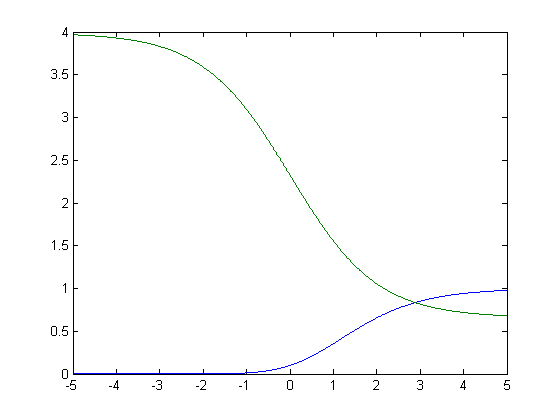
\includegraphics[width=0.8\textwidth]{sigmoidfigure}
    \label{sigmoid}
\end{figure}
The threshold multiplier is taken piece-wisely from the lower parts of the two functions, and it modifies $\xi$ according to its value. Although having this threshold makes the agent agree on bids that it would not accept, having just the acceptance threshold discussed in the previous subsection, modeling showed that taking opponent leaps into account increases the utility the agent receives by $5\dots10\%$ on average.

\subsection{Deciding on Acceptance}
Finally the agent's Acceptance Strategy is comprised of the following statement represented in pseudo-code below:
\begin{verbatim}
AcceptanceAction() {
   if(lastOpponentBidUtil <= weakThreshold * delta) {
       Reject();
   }
   if(isLeapBigEnough() 
     && lastOpponentBidUtil > getLeapTheshold()){
       Accept();
   }
   if(lastOpponentBidUtil >= acceptanceThreshold 
      or lastOpponentBidUtil >= pressureThreshold) {
       Accept();
   }
   Reject();
\end{verbatim}
Here \texttt{weakThreshold} is provided by the Opponent Model, which is described in the following section.

\section{Opponent Model}  

The Opponent Model is based on the \textit{Hard-Headed Model} from the BOA framework. The basic difference from the Hard-Headed Model lies in the way the weights are modified. They are updated only if the number of unique bids an opponent has made in the recent past is above a certain value. This is done to prevent fast convergence to suboptimal weights and thus wrong representation of the opponents behavior.

Classic Opponent Model in the NegoAgent was also enhanced with the module, which calculates a threshold that is based on the~\textit{Distance Of The Opponent in Our Utility Space}$-$\texttt{DOUS} value~\cite{anac2013}. This value is used in the Acceptance Strategy and provides the agent with a threshold that helps reject bids that are far from Nash, in high discount environments.

The basic algorithm of the DOUS value and its threshold calculation is the following:
\begin{verbatim}
double getDousThreshold(horizon){
    myUtility = negotiationSession.getMyMaxUtil();
    dous      = myUtility - getOpponentLastBid().getMyUtil();
    mean      = getOpponentBidsMean(horizon);
    variance  = getOpponentBidVar(horizon, mean);
    time      = getTime();
    threshold = (mean + dous)/2;
    if(time > timeLimit) {
        threshold += (1 - (time - 0.9)) * variance;
    }else {
        threshold += variance;
    }
    if(time > delta) {
        return 0;
    }    
    return threshold;
}
\end{verbatim}

The~\texttt{horizon} parameter, defines the number of past bids the agent takes into account when calculating the~\texttt{DOUS} distance. The smaller the~\texttt{horizon}, the more short-sighted the agent's threshold is. If the horizon is assigned a large value, the fluctuations of the bids' utilities will not be imprinted with the same precision at the output value, and this may result in a low threshold. Usually, the~\texttt{horizon} value lays between $10$ and $100$ efficient captures of the opponent bids' fluctuations.

Whenever the discount factor $\delta$ is a low, and the utility is greatly discounted over time, the threshold is kept for a short period of time. On the other hand, if $\delta$ is large, the threshold is kept for a prolonged time.

The~\texttt{DOUS} value is versatile, as is not domain dependent. The visualization of the DOUS distance is given in Fig.~\ref{DOUS}. As shown here, it can be implemented only in negotiations between two agents, but it can be expanded to multiple agent negotiations creating a~\texttt{DOUS} distance for every agent pair. 

The threshold that is outputted is a \texttt{weakThreshold}. If the utility value of a bid an opponent offers to the NegoAgent is smaller than the \texttt{weakThreshold}, the bid is rejected. If the value is higher, we compare it with the strong threshold computed in the Acceptance Strategy. This ensures that the agents rejects points that are far from the Nash equilibrium.

The amount of time this threshold holds is dependent on the $\delta$ of the negotiation domain. This restriction is set because the agent needs to be more concessive as the deadline approaches. If the discount factor is $1$, and no depreciation exists, this threshold stands for the whole negotiation. 
\begin{figure}[htbp]
  \caption{The distance between the initial utilities of the agents}
  \centering
    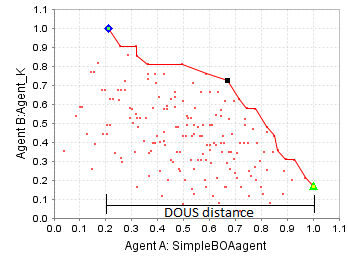
\includegraphics[width=0.5\textwidth]{dous}
    \label{DOUS}
\end{figure}

\section{Opponent Model Strategy}  

This module was adapted from a \textit{Best Bid Strategy}, included in Genius. The idea behind it is in keeping a small history of opponent's bids for determination of the best bid. An experimentation with a history size showed that keeping of the considerable amount of opponent's bids has a negative impact on the agent's performance, thus the history size was set to $10$ independent of the domain.

The most basic OMS was selected to show the strengths and weaknesses of the NegoAgent in its current state regardless or other variables introduced by more advanced models. However it is likely that a more tuned model is to increase the agent's performance, and thus this leaves a space for further investigation.

\section{Binding the Modules}

It is useful to have a single-entity agent instead of several BOA components. In particular, Genius allows single-entity agents run separate sessions against each other, and ANAC competition uses this kind of agents in the tournament series. A single-entity agent may consist of numerous parts, however the one described in the paper is comprised of four main BOA components, described in the previous sections.

In order to bind all the modules together, a class that extended the BOA agent and passes each of the modules with its parameters as parts of the agent should be created. Then it is necessary to override an \texttt{agentSetup} method of the class. The pseudo-code of the overriden class is:

\begin{verbatim}
NegoAgent extends BOAagent {    
    @Override
    agentSetup(){
        OpponentModel om = new OpponentsModel(negotiationSession);
        OMStrategy oms = new BidStrategy(negotiationSession , om);
        OfferingStrategy offering = new NegoAgent_TDOffering(nego-
        tiationSession, om, oms, Pmax, Pmin);
        AcceptanceStrategy ac =  new AStrategy(negotiationSession,
        offering, a , b, c);
        setDecoupledComponents (ac, offering, om, oms );
    }
}
\end{verbatim}

\section{Results}

The agent implemented is a strong-willed agent. It accepts bids fast when the depreciation is large, otherwise it negotiates a better deal until the end of a negotiation session. The Acceptance Strategy with the~\texttt{weakThreshold} restricts the agent from accepting offers that are not at least close to the Nash equilibrium. As $t\to1$, the~\texttt{weakThreshold} is dropped, and the acceptance threshold is reduced, making the agent capable of accepting more reasonable bids. Its TD offering makes the agent extremely efficient at obtaining the best utility possible from strong willed opponents. Table~\ref{table:NegoSimpleResults} shows the performance tests results of a proposed NegoAgent versus several existed agents ranging from most basic to the most advanced ones.

\begin{table}[htbp] 
	\centering % used for centering table 
	\caption{NegoAgent's negotiation results}
	\setlength{\tabcolsep}{0.5em}
	\begin{tabular}{llcccccc} % centered columns
		\toprule[0.15em] 
		 Opponent  &  Role (B) & Rounds & u, A & u, B & $\delta$u, A & $\delta$u, B & $t$\\ [0.5ex] % inserts table 
		\midrule 
		\multirow{2}{*}{Simple}&Mary&41&1&0.4500&0.9755&0.4390&0.1148\\
		&Sam&73&1&0.5250&0.9591&0.5035&0.1932\\ 
		\midrule
		\multirow{2}{*}{Meta}&Itex&6517&0.9268&0.3073&0.9268&0.3073&0.9822\\
		&Cypress&7475&0&0&0&0&1\\
		\midrule
		\multirow{2}{*}{TitfotTat}&CarA2&1406&0.9641&0.8936&0.7269&0.6737&0.9818\\
		&CarA1&1536&0.9800&0.7642&0.7360&0.5739&0.9953\\
		\midrule
		\multirow{2}{*}{Negotiator}&SmartP2&1145&0.9585&0.6635&0.8466&0.5861&0.8911\\
		&SmartP1&1061&0.9776&0.5540&0.8605&0.4877&0.9158\\
		\midrule
		\multirow{2}{*}{CUHKA}&NiceOrDie2&3681&0.2990&0.2990&0.2243&0.2243&0.9990\\
		&NiceOrDie1&3437&0.2990&0.2990&0.2243&0.2243&0.9986\\
		\bottomrule[0.15em] 
	\end{tabular}
	 
	\caption*{u - utility of agent, $\delta$u - discounted utility. Opponents negotiated for role B} 
	\label{table:NegoSimpleResults} % is used to refer this table in the text 
\end{table} 

In the first negotiation outcome, NegoAgent completely dominates over a \textit{SimpleAgent} in the domain Sam and Mary. An agreement is reached very fast, and the NegoAgent gathers the max amount of utility it can gather in this domain. 

In the second session, NegoAgent negotiates in the ItexVsCypress domain against the \textit{MetaAgent}. MetaAgent is not a normal agent; it contains an agent repository that consists of the agents that competed in the ANAC'2012, and uses machine learning to decide which agent fits best for each negotiation domain. It competed in the ANAC'2013 and took the second place. MetaAgent is completely defeated on the first session, whereas on the second, no agreement is reached.

In the third session, NegoAgent is opposed by a \textit{NiceTitForTat} agent in the car buyer-car seller domain. NiceTitForTat loses, but manages to keep the utility it gains from the session relatively high. In contrast to the SimpleAgent, the negotiation on both sessions took a lot of time.

In the fourth session, NegoAgent competes against \textit{Negotiator} agent in the Smartphone buying domain. Negotiator also looses against NegoAgent and, in contrast to NiceTitForTat, it does not manage to keep its utility high enough.

In the final session, NegoAgent is opposed by \textit{CUHKA} agent in the NiceOrDie domain. CUHKA agent is a very intelligent self-interested agent, and the agreement is reached at the Nash point of this domain. It must be noted that this domain has only 3 possible bids that can be offered, and the agreement is accepted on the final offer of our agent.

Finally, the screen shots taken from the Genius GUI, show the negotiation results of NegoAgent against different opponents in Fig.~\ref{sessionGraphs}.
\begin{figure}[htbp]
	\centering
	\captionsetup{justification=centering}
	\begin{minipage}{.3\textwidth}
		\centering
		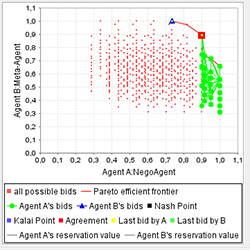
\includegraphics[width=.9\linewidth]{1}
		\caption*{a) vs. Meta Agent (Icecream)}
	\end{minipage}%
	\begin{minipage}{.3\textwidth}
		\centering
		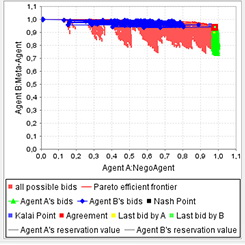
\includegraphics[width=.9\linewidth]{2}
		\caption*{b) vs. Meta Agent (Kitchen)}
	\end{minipage}
	\begin{minipage}{.3\textwidth}
		\centering
		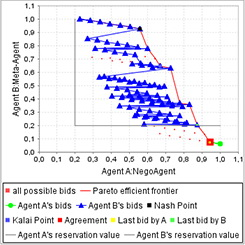
\includegraphics[width=.9\linewidth]{3}
		\caption*{c) vs. Meta Agent (Coffee)}
	\end{minipage} \\
	\begin{minipage}{.3\textwidth}
		\centering
		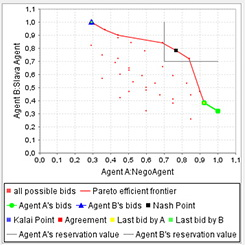
\includegraphics[width=.9\linewidth]{4}
		\caption*{d) vs. SlavaAgent (DefenciveCharms)}
	\end{minipage}
	\begin{minipage}{.3\textwidth}
		\centering
		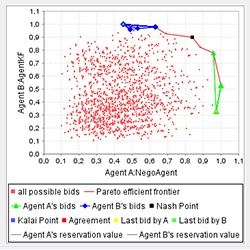
\includegraphics[width=.9\linewidth]{5}
		\caption*{e) vs. AgentKF (Grocery)}
	\end{minipage}
	\begin{minipage}{.3\textwidth}
		\centering
		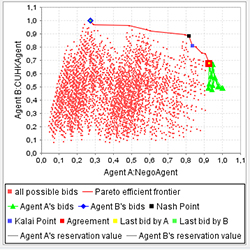
\includegraphics[width=.9\linewidth]{6}
		\caption*{f) vs. CUHKA (Camera)}
	\end{minipage}\\
	\begin{minipage}{.3\textwidth}
		\centering
		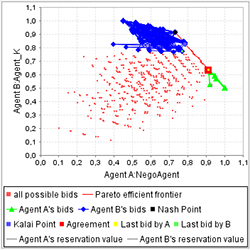
\includegraphics[width=.9\linewidth]{7}
		\caption*{j) vs. Agent$\_$K (EnglandVsZimbabwe)}
	\end{minipage}
	\begin{minipage}{.3\textwidth}
		\centering
		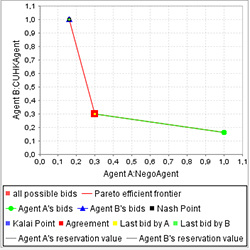
\includegraphics[width=.9\linewidth]{8}
		\caption*{k) vs. CUHKA (NiceOrDie)}
	\end{minipage}
	\caption{Nego Agent negotiation sessions' results. \\Negotiation domain name is given in brackets}
	\label{sessionGraphs}
\end{figure}

It can be seen how the agent extracts more utility from its opponents within domains similar to the ones shown in Fig.~\ref{sessionGraphs} b) and j), where NegoAgent is proposed a bid and accepts it, while an opponent loses a significant amount of utility on this bid. There are also cases like shown in Fig.~\ref{sessionGraphs} a) and f), where NegoAgent proposes a bid which is accepted by its opponents, overpowering their opposition. It can also be noted that in Fig.~\ref{sessionGraphs} b), in a three possible bids domain, the agent proposes an optimal bid which is at Nash, and waits for the CUHKA agent to accept it. Finally, as shown in Fig.~\ref{sessionGraphs} d) and e), there are cases where the agents do not reach an agreement since no side is willing to bid less, and no side agrees on any of the opposing bids.

\section{Conclusion}
Building a negotiating agent is a non-trivial matter, as the negotiation domains and issue sets are practically infinite, so are the strategies that can be used. Negotiation agent design is an active research field that has been introduced recently, thus very limited practical experience is shared yet. The proposed NegoAgent tries to incorporate some of the Multi-Agent Systems concepts in it's negotiation behavior. Some domain/opponent specific cases might be treated separately, but it was decided to as general and versatile as possible. Overall results the NegoAgent shows against competitive opponents are promising, and the agent is believed to be a solid base for further research. 

\begin{thebibliography}{}

\bibitem{abines} 
Hao J.Y., Leung H.F.:
ABiNeS: An Adaptive Bilateral Negotiating Strategy over Multiple Items,
Proc WI-IAT, 95--102 (2012)

\bibitem{genius}
Genius platform at TU Delft,
\texttt{http://www.mmi.tudelft.nl/genius/} Retrieval date: 01.12.13

\bibitem{anac2013}
Fourth Automated Negotiating Agent Competition (2013).:
\texttt{http://www.itolab.nitech.ac.jp/ANAC2013/} Retrieval date: 01.12.13

\end{thebibliography}

\end{document}